\documentclass[11pt]{article}   % list options between brackets
\usepackage{graphicx}  % most common package for figure handling
\usepackage{amsmath}  
\usepackage{amssymb}
\usepackage{url}
\usepackage{verbatim} % useful for displaying computer code or similar verbatim
\usepackage{full page} % This package changes the otherwise very generous margins to 1 inch on all sides
\usepackage{float}
\usepackage{listings}
\usepackage{amsmath}
\usepackage{bigstrut}
\usepackage{rotating}
\usepackage{hyperref}
\usepackage{pdflscape }
\usepackage{program}
\usepackage[framed,numbered,autolinebreaks,useliterate]{mcode}

 \usepackage{algpseudocode}
\usepackage{subfig}
\begin{document}
\setlength{\parindent}{0.00in}
%\ttfamily

\title{EN2202 Assignment 1}

\author{
 Sam Lewis\\
 svrlewis@kth.se
  \and
  Bjoern Fischer  
}
\date{} 
\maketitle
\linespread{1.5}

\section{Verification of the Markov chain random code}

Considering the infinite duration HMM $\lambda = {q, A, B}$ with

$$q =\begin{pmatrix} 0.75 \\ 0.25 \end{pmatrix} ;  A = \begin{pmatrix} 0.99 & 0.01 \\ 0.03 & 0.97 \end{pmatrix} $$

The $q$ vector defines the initial state probability, that is  
$$P_1 = \begin{pmatrix} P(S_1 = 1) \\ P(S_1 = 2) \end{pmatrix} = q =\begin{pmatrix} 0.75 \\ 0.25 \end{pmatrix}  $$

For the next time step, $t = 2$ the transition probability matrix can be used to find the new state probabilities. 

$$P_2 = \begin{pmatrix} P(S_2 = 1) \\ P(S_2 = 2) \end{pmatrix} = (q^TA)^T = 
(\begin{pmatrix} 0.75  & 0.25 \end{pmatrix} \begin{pmatrix} 0.99 & 0.01 \\ 0.03 & 0.97 \end{pmatrix})^T =  \begin{pmatrix} 0.75 \\ 0.25 \end{pmatrix}  $$\

Because the transition matrix for the Markov chain is constant for all time t, this means that the state probability is also constant for all time t, and is equal to $q$. \\

This was verified using the \texttt{rand} of the the Markov Chain class to generate a sequence of 10000 states using the following MATLAB script.

\begin{lstlisting}
mc = MarkovChain([0.75; 0.25], [0.99 0.01 ; 0.03 0.97]);
S = rand(mc, 10000);

state1 = sum(S == 1)
state2 = sum(S == 2)
\end{lstlisting}\

Running this script once gave the result of \texttt{state1 = 7598; state2 =  2402} which is close to the expected distribution.

\newpage

\section{Verification of the HMM random code}

For the system, listed above the expected value and variance can both be theoretically found.

$$ E[X_T] = E_S [E_x[X \mid S]] = \Pr(S = 1)  E_x[X \mid S = 1] + P(S = 2)E_x[X \mid S = 2] = 0.75 \cdot 0 + 0.25 \cdot 3 = 0.75$$ 

$$ \newcommand{\Var}{\mathrm{Var}} \begin{array} {lcl} \Var[x] & = & E_S [ \Var_x [ X \mid S]] + \Var_s [E_x [X \mid S] ] \\ 
& = & \Pr(S = 1) \Var_x [X \mid S = 1] + \Pr(S = 2) \Var_x[X \mid S = 2] \\
 & + & \Pr(S = 1) (E_x[X \mid S = 1] - \mu)^2 + \Pr(S = 2)(E_x[X \mid S = 2] - \mu)^2\\
 & = & 0.75 \cdot 1^2 + 0.25 \cdot 2^2 + 0.75(0 - 0.75)^2 + 0.25(3- 0.75)^2 \\
 & = & 3.4375 \end{array}$$

The following script was then used to verify the theoretical results.

\begin{lstlisting}
mc = MarkovChain([0.75; 0.25], [0.99 0.01 ; 0.03 0.97]);
b1 = GaussD('Mean', 0, 'StDev', 1);
b2 = GaussD('Mean', 3, 'StDev', 2);
h = HMM(mc, [b1 ; b2]) ;
[X, S] = rand(h, 10000);
mean(X)
var(X)
\end{lstlisting}\

This script gave the mean to be 0.7315 and the variance 3.3367, again close to the expected results.
\newpage

\section{HMM behaviour}

For the HMM listed in section 1, 500 random contiguous output samples were plotted together with the state that the HMM was in.

\begin{figure}[H]
\begin{center}
\leavevmode
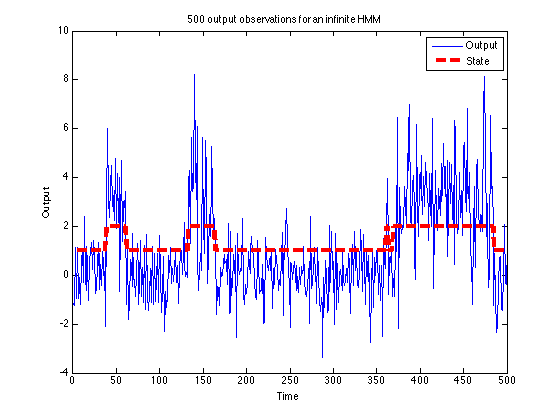
\includegraphics[width=1\textwidth]{infiniteHMMoutput.png}
\end{center}
\caption{500 random output observations from the HMM described in section 1. The blue line is the output from the HMM while the red dotted line is the state that the HMM is in.}
\label{euler:1}
\end{figure}

It is clear from the picture that in the second state, the output is around 3 and in the first state the output is around 0. The second state output has a larger variation, because the standard deviation of the Gaussian for the second state is larger than that of the first state. \\
\newpage
The output distributions for the HMM were then altered so that the mean of the output distribution for each state was 0. Again, 500 samples were plotted and the result is shown in figure 2. 

\begin{figure}[H]
\begin{center}
\leavevmode
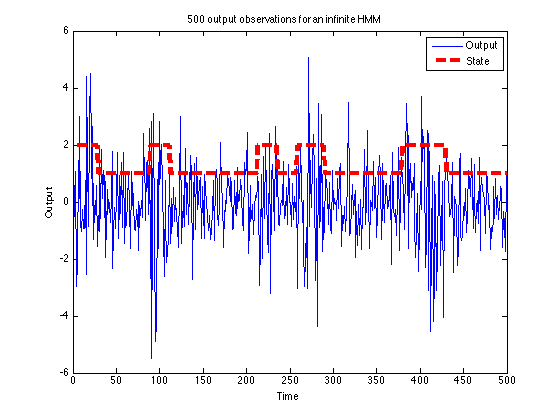
\includegraphics[width=1\textwidth]{identicalMeanHMM.png}
\end{center}
\caption{500 random output observations from the HMM described in section 1 with $\mu_1 = \mu_2 = 0$}
\label{euler:1}
\end{figure}

This time it is harder to distinguish the state sequence purely from looking at the output from the HMM. However, when the state is state 2, the standard deviation is higher so the output range is larger. This helps in identifying the state sequence but it is still more difficult than the previous model.

\newpage

\section{Finite HMM verification}

To test finite duration HMMs the HMM from section 1 was modified so that..\\

 $$A = \begin{pmatrix} 0.89 & 0.01 & 0.1\\ 0.03 & 0.87 & 0.1 \end{pmatrix} $$\\
 
This means that  the probability of the state sequence terminating is always 0.1, so on average a state sequence should terminate after 10 steps. The following script was written to test this practically.

\begin{lstlisting}
mc = MarkovChain([0.75; 0.25], [0.89 0.01 0.1; 0.03 0.87 0.1]);

b1 = GaussD('Mean', 0, 'StDev', 1);
b2 = GaussD('Mean', 3, 'StDev', 2);

h = HMM(mc, [b1 ; b2]) ;

tests = 1000;
average = 0;

for i=1:tests
    [X, S] = rand(h, 500);
    average = average + length(X);
end

average/tests
\end{lstlisting}\
 
 This resulted in an average sequence length of 9.94, very close to what was expected.
 
\newpage
\section{Vector valued HMM verification}

To verify that the HMM code worked for when the output distributions generate random vectors the following code was used.

\begin{lstlisting}mc = MarkovChain([0.75; 0.25], [0.99 0.01 ; 0.03 0.97]);

mean1 = [1 2];
mean2 = [5 7];

cov1 = [1 0; 0 1];
cov2 = [2 1; 1 4];

b1 = GaussD('Mean', mean1, 'Covariance', cov1);
b2 = GaussD('Mean', mean2, 'Covariance', cov2);

h = HMM(mc, [b1 ; b2]) ;

[X, S] = rand(h, 500);
\end{lstlisting}\

This worked as expected, with the X output vector consisting of feature vectors of length 2.

\end{document}


